\chapter[Bakgrunn]{Bakgrunn}
\label{ch:background}
\blindtext

\section{Velferdsteknologi}
\citet{regjeringen_hagen} er en norsk offentlig utredning (NOU) om velferdsteknologi med tittelen «Innovasjon i omsorg».
Utredningen benytter følgende definisjon av velferdsteknologi:

\blockquote{
Med velferdsteknologi menes først og fremst
teknologisk assistanse som bidrar til økt trygghet,
sikkerhet, sosial deltakelse, mobilitet og
fysisk og kulturell aktivitet, og styrker den
enkeltes evne til å klare seg selv i hverdagen til
tross for sykdom og sosial, psykisk eller fysisk
nedsatt funksjonsevne. Velferdsteknologi kan
også fungere som teknologisk støtte til pårørende og
ellers bidra til å forbedre tilgjengelighet,
ressursutnyttelse og kvalitet på tjenestetilbudet.
Velferdsteknologiske løsninger kan i
mange tilfeller forebygge behov for tjenester
eller innleggelse i institusjon.
}

\begin{figure}
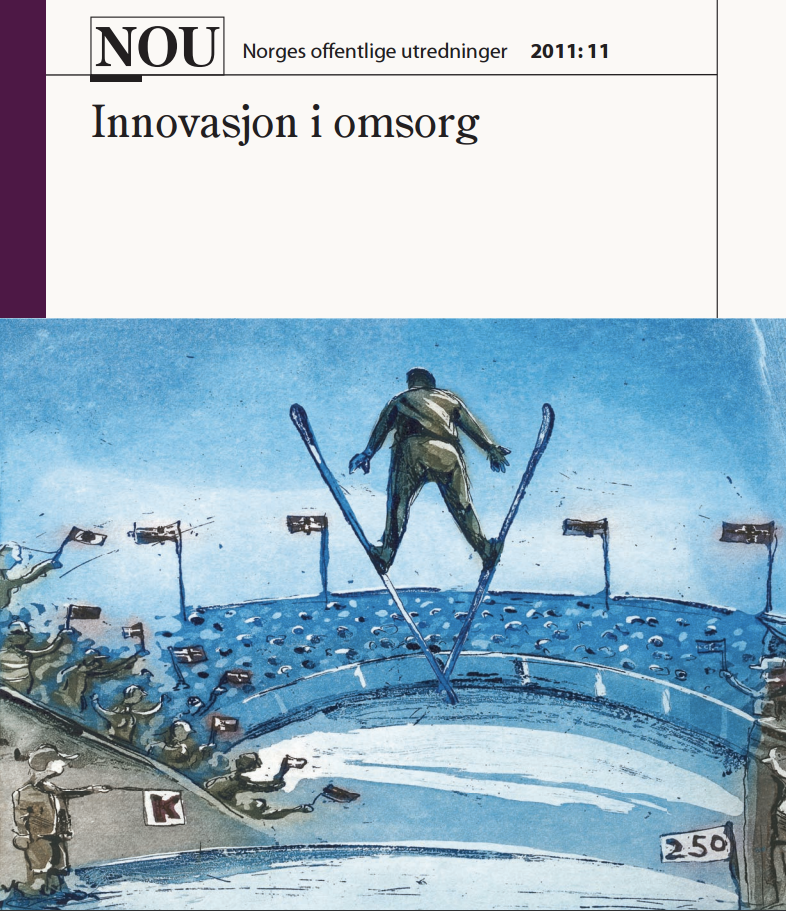
\includegraphics[width=0.85\textwidth,center]{fig/hagen}
\caption{Hagen-komiteen: Siden 2011 har det blitt hoppet over 250 meter i Vikersund, og verdensrekorden er nå 253,5 meter. }
\label{fig:hagen}
\end{figure}

\citet{regjeringen_hagen} anbefaler fem punkter for myndighetene å fokusere på i fremtiden:

\begin{enumerate}
    \item «Næromsorg» -- den andre samhandlingsreformen: mobiliser ressurser i samarbeid med
    lokalsamfunnet, det sosiale nettverket til pasienten og familien.
    \item «Teknoplan 2015» -- teknologistøtte til omsorg: bruk ny og eksisterende teknologi for å gi brukere
    bedre trygghet og muligheten til å bo hjemme og motta støtte.
    \item «Nye rom» -- fremtidens boligløsninger og nærmiljø: boliger og leiligheter må tilpasses eldre.
    \item Et nasjonalt program for kommunal innovasjon i omsorg: kommunene har hovedansvaret for omsorgstjenester,
    og myndighetene kan støtte kommunene med incentiver til nye løsninger.
    \item Omsorgsfeltet som næring: Norge kan være en ledende nasjon i utviklingen av nye omsorgsprodukter, og
    eksportere disse innovasjonene. Omsorgsfeltet åpnes opp for importering av eksportering av varer og tjenester.
\end{enumerate}

Spesielt teknoplan og nasjonalt program er interessant for denne oppgaven blabla (skrive noe mer om de to punktene).

Stortingsmeldingen «Morgendagens omsorg» bygger på arbeidet til \citet{regjeringen_hagen} \citet{morgendagens_omsorg}.
I denne meldingen legger regjeringen frem «Omsorgsplan 2020» som inkluderer et program for velferdsteknologi de neste årene.
Ett av initiativene i programmet er å bygge og etablere åpne velferdsteknologistandarder. Dette vil lette integreringen av nye
løsninger i privat og offentlig sektor. Andre initiativer er å utvikle og teste velferdsteknologiløsninger i kommunene,
bygge og dele kunnskap og lage modeller og rammeverk som andre kan bruke.

In the revised national budget for 2014, the Storting allocated money for a national welfare technology program. The
five priority initiatives in the program are: (1) Safety and sense of achievement at home, (2) Remote monitoring of
people with chronic diseases, (3) mHelse, (4) Social networks - reduce and counteract loneliness in the elderly, and (5)
facilitate that children and youth with disabilities can be more active.

According to \citet{welfare_ethical}, welfare technology has a moral end. It is supposed to
e.g. give better and more focused care, and reduced risk and increased safety for people. See table
\ref{table:welfare_definition} for different applications of welfare technology. 

\newcolumntype{C}{>{\Centering\arraybackslash}X} % centered "X" column

\begin{table}[!ht]
\setlength\extrarowheight{2pt} % for a bit of visual "breathing space"
\centering
\begin{tabularx}{\textwidth}{|X|X|}
\hline
\textbf{Technology/purpose} & \textbf{Examples/function} \\ \hline
Communication support & Technologies for real time audio-visual contact \\ \hline
 & Physical Activity Monitoring for Aging People (PAMP) \\ \hline
 & Patient information (web-based, interactive) \\ \hline
Compensatory technology, assistive technology & Safety systems (alarms for heat, light, locking doors);
  security alarms; fall detector \\ \hline
  & Alarm systems (sound, light, vibration) \\ \hline
  & Mobility technologies, advanced rollators,wheelchairs for staircases, \\ \hline
Help to every day practical tasks & Housekeeping (making food, (vacuum) cleaning, tidying) \\ \hline

\end{tabularx}
\caption{Welfare technology classified according to purpose and function. \citep{welfare_ethical}}
\label{table:welfare_definition}
\end{table}


\section{Avstandsoppfølging av kronisk syke}
\blindtext

\section{Eldre pasienter og IT}
\blindtext

\section{Tingenes Internett}
\citet{iot_legal} define Internet of Things as "an emerging global
Internet-based information architecture facilitating the exchange of
goods and services". Therein lies a vision of a connected world of objects
communicating with each other. Multiple definitions of IoT exist depending on the business domain.
\citet{iot_harvard_smart} writes that the phrase "Internet of Things" is not a very good description
of the new era of interconnected devices:

\blockquote{\enquote{What makes smart, connected products fundamentally different is not the internet,
but the changing nature of the “things.” It is the expanded capabilities of smart, connected
products and the data they generate that are ushering in a new era of competition.}}

Therefore, they coin the term "smart products" which comprise three elements:

\begin{itemize}
    \item Physical components: the electrical and mechanical parts of the product.
    \item "Smart" components: sensors, processors, software, operating system, storage, user interface.
    \item Connectivity components: ports, antennae, protocols enabling wired/wireless connections
    one-to-one, one-to-many, many-to-many.
\end{itemize}
Smart products introduce a new technology stack (figure \ref{fig:iot_harvard_smart}), with products connected to a product cloud.
The product cloud includes a big-data database system, and a rules/analytics engine to run business logic efficiently,
and utilize and analyze all the information from the products. These smart, connected products have four capabilities building
on each other (figure \ref{fig:iot_harvard_capabilities}): Monitoring, control, optimization and autonomy.
Tesla is an example of a smart product combining monitoring, control and optimization to allow autonomy. The car itself performs
self-diagnosis, and updates automatically without external car service.

\citet{iot_harvard_smartcompanies} suggests that smart, connected products are transforming companies as well, by altering
every step in value chain. The utilization of data is more important, and product design is not only a mechanical venture,
but an interdisciplinary journey which requires more software engineering.

\begin{figure}
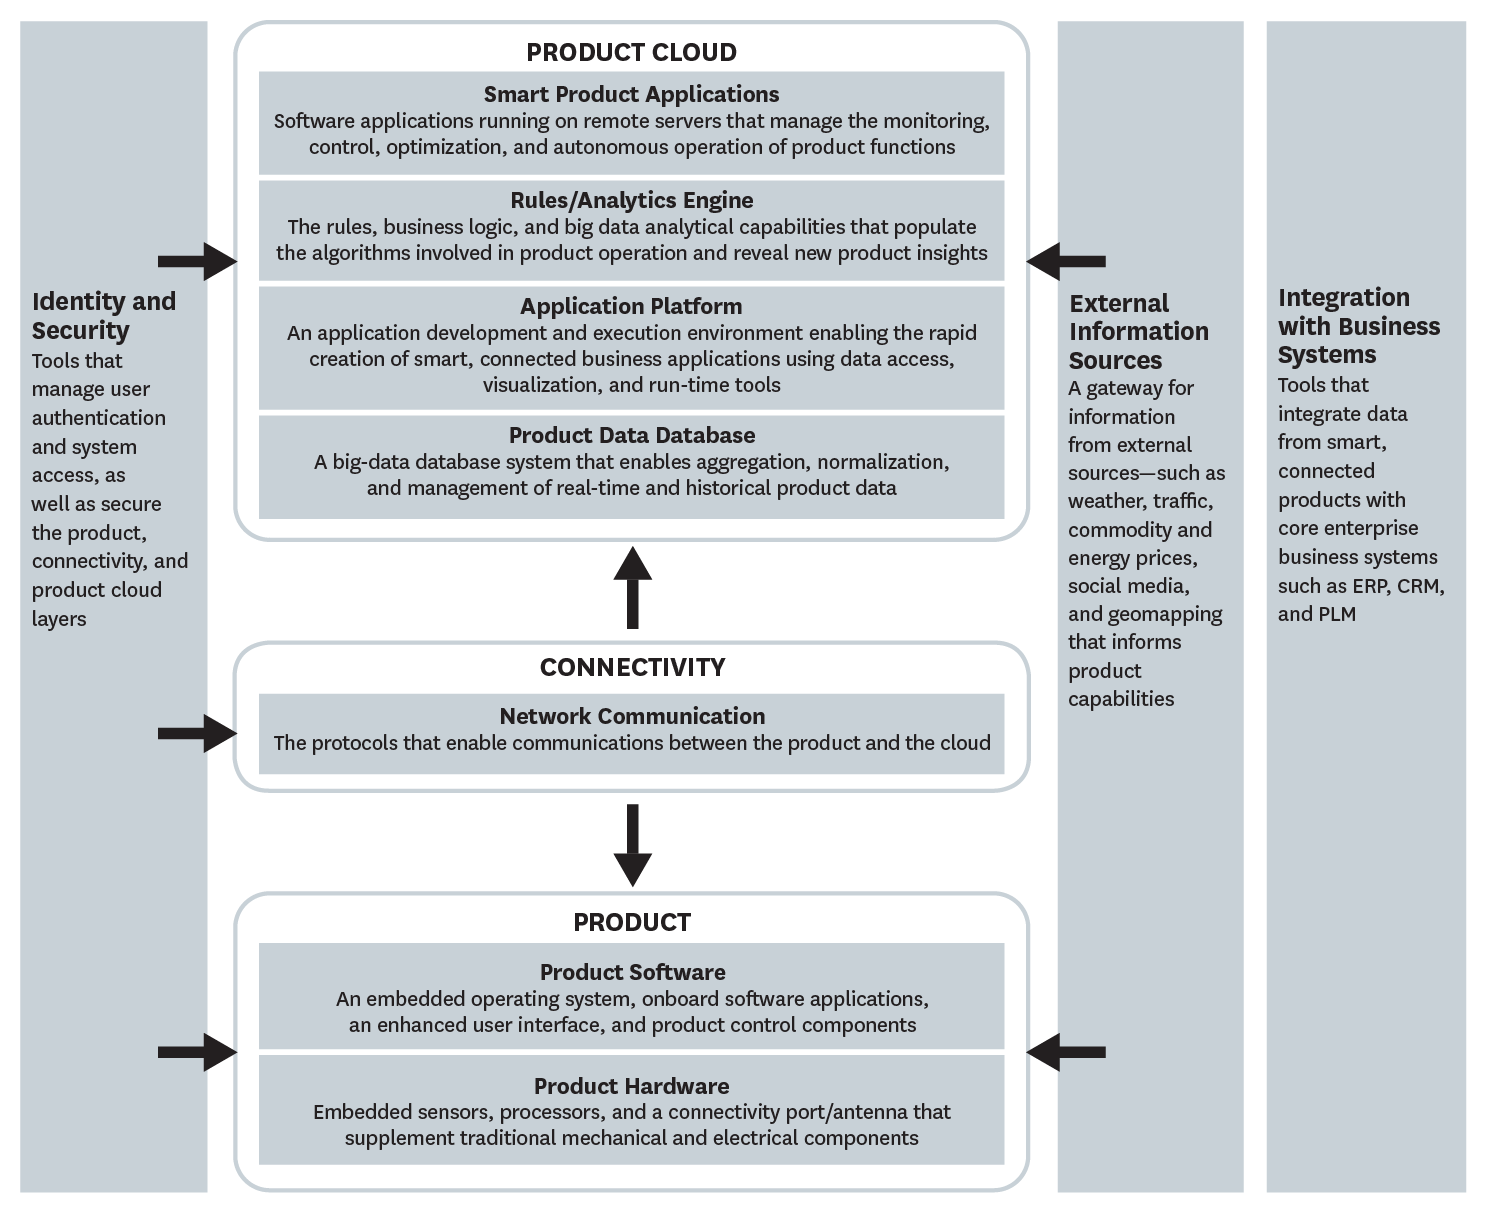
\includegraphics[width=1.1\textwidth,center]{fig/harvard_technology}
\caption{The new technology stack \citep{iot_harvard_smart}}
\label{fig:iot_harvard_smart}
\end{figure}

\begin{figure}
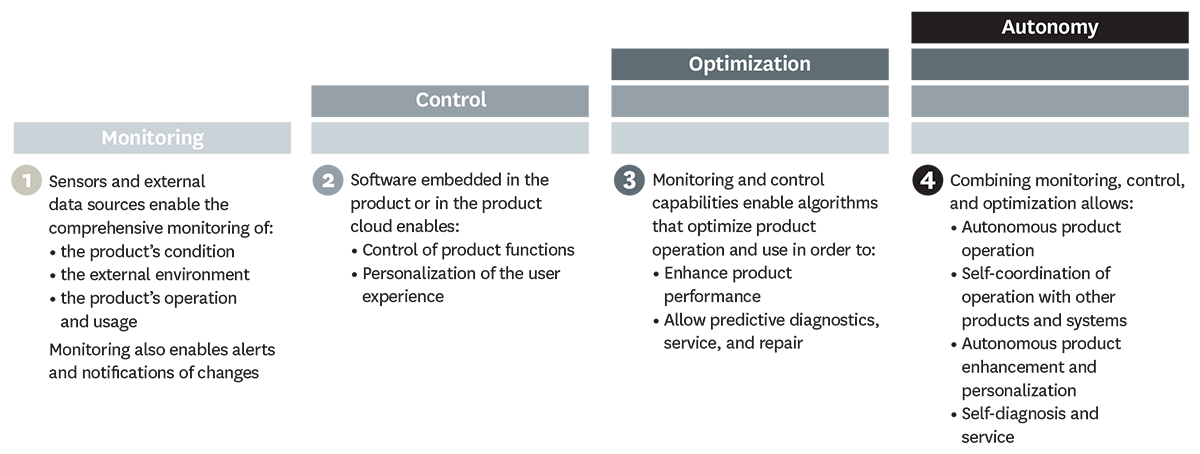
\includegraphics[width=1.1\textwidth,center]{fig/harvard_capabilities}
\caption{Capabilities of smart products \citep{iot_harvard_smart}}
\label{fig:iot_harvard_capabilities}
\end{figure}


\subsection{Sikkerhet i tingenes internett}
Experts have raised concerns regarding the security model of IoT. On October 21, 2016, the Internet core
infrastructure company \textit{Dyn} was attacked by millions of small devices (mainly routers and cameras)
with small to none security \citep{iot_attack_ddos}. This affected several large websites such as Twitter,
Spotify, and PayPal. Routers and web cameras often ship with common default passwords that users
do not change, and can be remotely accessed through common ports (22/SSH, 80/HTTP, 23/Telnet)
\citep{iot_mirai_botnet}. 

\citet{iot_schneier_regulation} calls for the government to impose regulations on IoT. He argues that
the markets fail to protect the security of the consumers. The consumers do not care, the manufacturers
do not care, and the products can never be patched after they are shipped and sold. However,
he emphasizes that the discussion about regulations should be made proactively, and not
after an IoT disaster where feelings are heated.

\section{Tingenes Internett i velferdsteknologi}
Personal Connected Health Alliance (PCHA) publishes the Continua Design Guidelines every year,
an open framework for end-to-end interoperability of personal connected health devices and systems \citep{continua_guidelines}.
An overview of the Continua framework can be found in figure \ref{fig:continua}. Personal devices
communicate with protocols like Bluetooth or Zigbee to a hub (Personal Area Network), and the hub sends information
to a Telehealth Service Center. From there, the data can be transmitted to health records.


As part of Care plan 2020 and National program for welfare technology, the government decided
in late 2014 that the Continua framework should be the foundation for every
welfare technology solution in Norway, on recommendation from the Norwegian Health Directorate \citep{regjeringen_continua}.
The standardization framework makes sure that different solutions work well together.

\begin{figure}
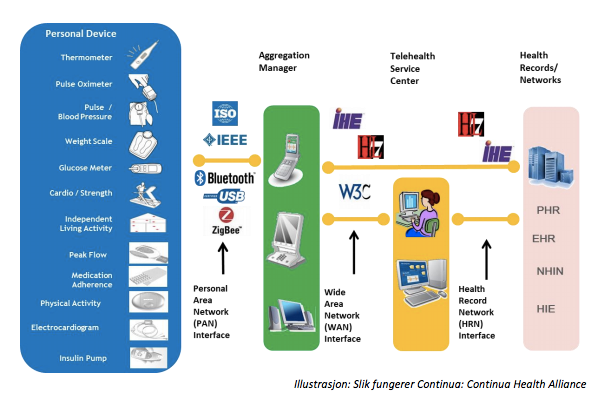
\includegraphics[width=0.9\textwidth,center]{fig/continua}
\caption{Continua framework overview}
\label{fig:continua}
\end{figure}
